\documentclass[a4paper,12pt]{article}
\usepackage[utf8]{inputenc}
\usepackage[MeX]{polski}
\usepackage{fixltx2e}            %textsubscript
\usepackage{graphicx}

%%%%%%%%%%%%%%%%%%%%%%%%%%%%%%%%%%%%%%%%%%%%%%%%%%%%%%%%%%%%%STRONA TYTUlOWA%%%%%%%%%%%%%%%%%%%%%%%%%%%%%%%%%%%%%%%%%%%%%%%%%%%%%%%%%%%%%%%%%%%%%%%%
\title{\Huge \textbf{Politechnika Wrocławska\\[0.3in]} 
  \huge Katedra Teorii Pola, Układów elektronicznych i Optoelektronicznych \\[0.2in]
  \LARGE Zespół Układów Elektronicznych
}
\date{}
\author{}
\begin{document}
\maketitle
\begin{table}[h]
  \large
  \centering
  \begin{tabular}{|ll|l|}
    \hline
    \multicolumn{1}{|l|}{Data: 21.04.2015r}                & \multicolumn{2}{l|}{Dzień: Wtorek}                                         \\ \hline
    \multicolumn{1}{|l|}{Grupa: VII}                      & \multicolumn{2}{l|}{Godzina: 12:15-15:00}                                  \\ \hline
    \multicolumn{3}{|l|}{\textit{\begin{tabular}[c]{@{}l@{}}\textbf{Temat ćwiczenia:} \\ Przerzutnik astabilny ``555''\end{tabular}}} \\ \hline
    \textbf{Dane projektowe:}                             & \multicolumn{2}{l|}{}                                                      \\
    T=0.50 \mu s                                          & \multicolumn{2}{l|}{}                                                      \\
    C=4.7 nF                                               & \multicolumn{2}{l|}{}                                                      \\
    R\textsubscript{a}=10k \Omega                         & \multicolumn{2}{l|}{}                                                      \\ \hline
    \multicolumn{1}{|l|}{\textbf{l.p}}                    & \textbf{Nazwisko i imię}                 & \textbf{Oceny}                  \\ \hline
    \multicolumn{1}{|l|}{1}                               & Arkadiusz Ziółkowski                     &                                 \\ \hline
    \multicolumn{1}{|l|}{2}                               & Jakub Koban                              &                                 \\ \hline
  \end{tabular}
\end{table}
%%%%%%%%%%%%%%%%%%%%%%%%%%%%%%%%%%%%%%%%%%%%%%%%%%%%%%%%%%%%%%%%%%%%%%%%%%%%%%%%%%%%%%%%%%%%%%%%%%%%%%%%%%%%%%%%%%%%%%%%%%%%%%%%%%%%%%%%%%%%%%%%%%%%
%%%%%%%%%%%%%%%%%%%%%%%%%%%%%%%%%%%%%%%%%%%%%%%%%%%%%%%%%%%%%%%%%%%ZADANIE PROJEKTOWE%%%%%%%%%%%%%%%%%%%%%%%%%%%%%%%%%%%%%%%%%%%%%%%%%%%%%%%%%%%%%%%
%%%%%%%%%%%%%%%%%%%%%%%%%%%%%%%%%%%%%%%%%%%%%%%%%%%%%%%%%%%%%%%%%%%%%%%%%%%%%%%%%%%%%%%%%%%%%%%%%%%%%%%%%%%%%%%%%%%%%%%%%%%%%%%%%%%%%%%%%%%%%%%%%%%%
\pagebreak
\section{Zadanie projektowe}
Zaprojektować przerzutnik monostabilny w oparciu o uład scalony ``555'' dla T=50 \mu s
%%%%%%%%%%%%%%%%%%%%%%%%%%%%%%%%%%%%%%%%%%%%%%%%%%%%%%%%%%%%%%%%%%%%%%%%%%%%%%%%%%%%%%%%%%%%%%%%%%%%%%%%%%%%%%%%%%%%%%%%%%%%%%%%%%%%%%%%%%%%%%%%%%%%
%%%%%%%%%%%%%%%%%%%%%%%%%%%%%%%%%%%%%%%%%%%%%%%%%%%%%%%%%%%%%%%%%%%CZĘŚĆ PROJEKTOWA%%%%%%%%%%%%%%%%%%%%%%%%%%%%%%%%%%%%%%%%%%%%%%%%%%%%%%%%%%%%%%%%%
%%%%%%%%%%%%%%%%%%%%%%%%%%%%%%%%%%%%%%%%%%%%%%%%%%%%%%%%%%%%%%%%%%%%%%%%%%%%%%%%%%%%%%%%%%%%%%%%%%%%%%%%%%%%%%%%%%%%%%%%%%%%%%%%%%%%%%%%%%%%%%%%%%%%
\subsection{Obliczenia projektowe}
\begin{equation}
  T=R_A\cdot C\cdot ln\left(\frac{V_{CC}}{V_{CC}-\frac{2}{3}V_{CC}}\right)\approx 1.1\cdot R_A\cdot C=1.1\cdot10k\Omega\cdot47nF = 51.7\mu s
\end{equation}
%%%%%%%%%%%%%%%%%%%%%%%%%%%%%%%%%%%%%%%%%%%%%%%%%%%%%%%%%%%%%%%%%%%%%%%%%%%%%%%%%%%%%%%%%%%%%%%%%%%%%%%%%%%%%%%%%%%%%%%%%%%%%%%%%%%%%%%%%%%%%%%%%%%%
\subsection {Schemat projektowy}   
\begin{figure}[h]
  \center 
  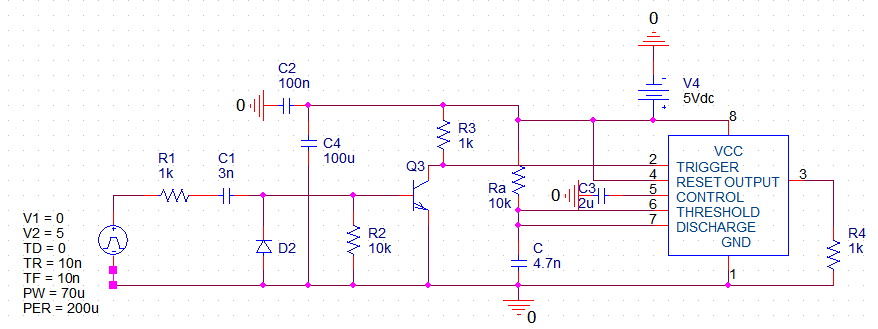
\includegraphics[width=1.1\textwidth]{schemat}
  \caption{Schemat projektowanego układu}
\end{figure}
\pagebreak
\subsection {Wyniki symulacji}   
\begin{figure}[h]
  \center 
  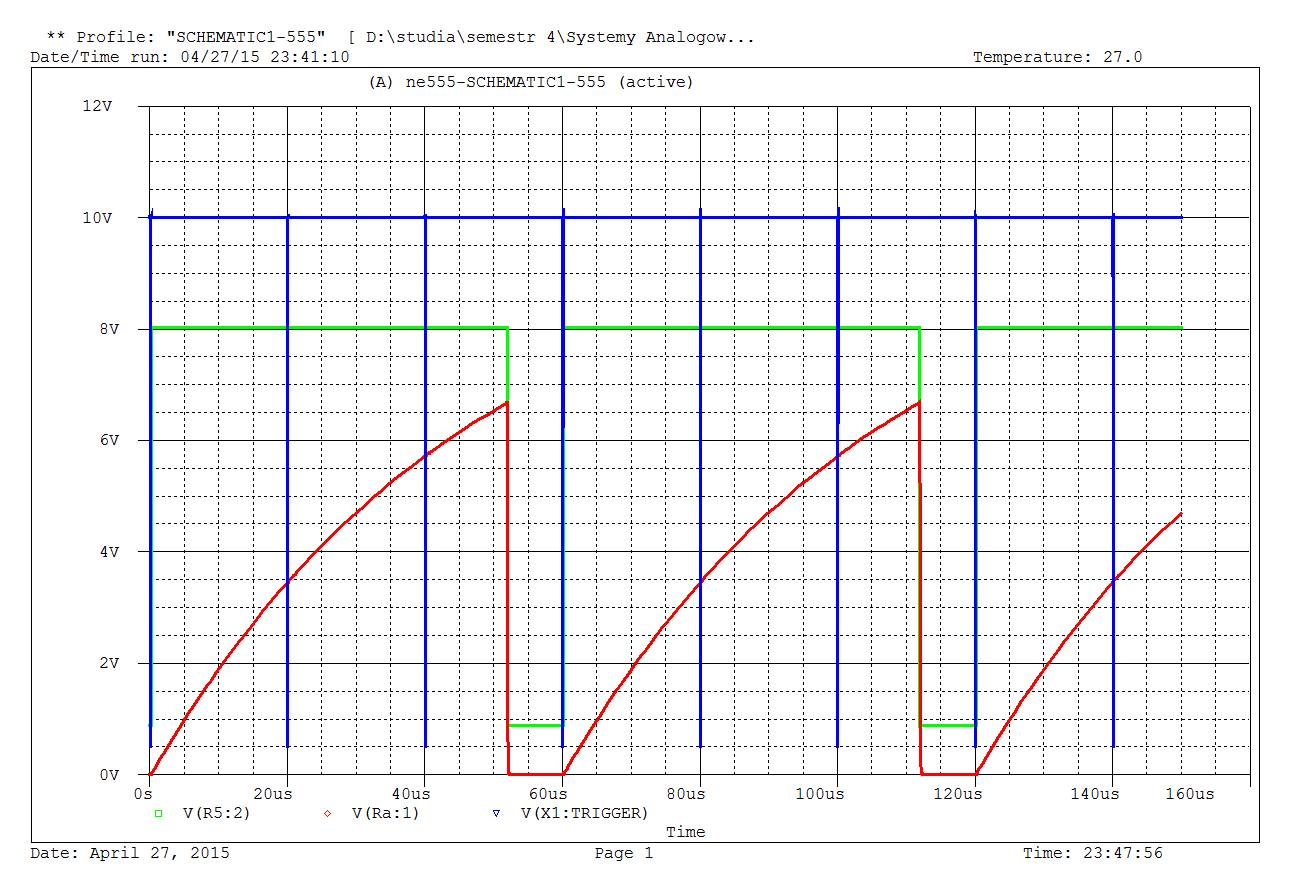
\includegraphics[width=1.2\textwidth]{sim}
  \caption{Wyniki symulacji}
\end{figure}
\begin{enumerate} 
\item Niebieski - napięcie wyzwalające  
\item Zielony - napięcie na wyjściu układu    
\item Czerwony - napięcie na kondensatorze
\end{enumerate}
%%%%%%%%%%%%%%%%%%%%%%%%%%%%%%%%%%%%%%%%%%%%%%%%%%%%%%%%%%%%%%%%%%%%%%%%%%%%%%%%%%%%%%%%%%%%%%%%%%%%%%%%%%%%%%%%%%%%%%%%%%%%%%%%%%%%%%%%%%%%%%%%%%%%
%%%%%%%%%%%%%%%%%%%%%%%%%%%%%%%%%%%%%%%%%%%%%%%%%%%%%%%%%%%%%%%%%%%CZĘŚĆ LABORATORYJNA%%%%%%%%%%%%%%%%%%%%%%%%%%%%%%%%%%%%%%%%%%%%%%%%%%%%%%%%%%%%%%
%%%%%%%%%%%%%%%%%%%%%%%%%%%%%%%%%%%%%%%%%%%%%%%%%%%%%%%%%%%%%%%%%%%%%%%%%%%%%%%%%%%%%%%%%%%%%%%%%%%%%%%%%%%%%%%%%%%%%%%%%%%%%%%%%%%%%%%%%%%%%%%%%%%%
\pagebreak
\section{Część laboratoryjna}
\subsection{Tabele pomiarowe}
\begin{figure}[!h]
\centering
\resizebox{\textwidth}{!}{%
\begin{tabular}{|c|c|c|l|l|l|c|c|}
\cline{1-3} \cline{7-8}
T[$\mu$ s]     & V\textsubscript{cc} [V]  & Odchylenie [$\%$] & \multicolumn{3}{l|}{\multirow{}{}{}} & T[$\mu$ s] &U\textsubscript{mod} [V]
\\ \cline{1-3} \cline{7-8} 
52.31 & 2.61  & 2.41       & \multicolumn{3}{l|}{}                   & 17.51               & 0.97              \\ \cline{1-3} \cline{7-8} 
51.62 & 3.03  & 1.06       & \multicolumn{3}{l|}{}                   & 18.14               & 1.48              \\ \cline{1-3} \cline{7-8} 
51.26 & 3.50  & 0.35       & \multicolumn{3}{l|}{}                   & 20.92               & 1.76              \\ \cline{1-3} \cline{7-8} 
51.14 & 3.99  & 0.12       & \multicolumn{3}{l|}{}                   & 24.80               & 2.05              \\ \cline{1-3} \cline{7-8} 
51.10 & 4.50  & 0.04       & \multicolumn{3}{l|}{}                   & 27.46               & 2.22              \\ \cline{1-3} \cline{7-8} 
51.08 & 5.02  & 0.00       & \multicolumn{3}{l|}{}                   & 32.37               & 2.52              \\ \cline{1-3} \cline{7-8} 
51.07 & 5.50  & -0.02      & \multicolumn{3}{l|}{}                   & 36.09               & 2.72              \\ \cline{1-3} \cline{7-8} 
51.06 & 5.99  & -0.04      & \multicolumn{3}{l|}{}                   & 42.66               & 2.99              \\ \cline{1-3} \cline{7-8} 
51.06 & 6.54  & -0.04      & \multicolumn{3}{l|}{}                   & 46.86               & 3.21              \\ \cline{1-3} \cline{7-8} 
51.07 & 7.02  & -0.02      & \multicolumn{3}{l|}{}                   & 54.60               & 3.50              \\ \cline{1-3} \cline{7-8} 
51.07 & 7.57  & -0.02      & \multicolumn{3}{l|}{}                   & 60.99               & 3.70              \\ \cline{1-3} \cline{7-8} 
51.08 & 7.99  & 0.00       & \multicolumn{3}{l|}{}                   & 71.96               & 4.00              \\ \cline{1-3} \cline{7-8} 
51.09 & 8.49  & 0.02       & \multicolumn{3}{l|}{}                   & 82.09               & 4.21              \\ \cline{1-3} \cline{7-8} 
51.11 & 9.07  & 0.06       & \multicolumn{3}{l|}{}                   & 92.35               & 4.56              \\ \cline{1-3} \cline{7-8} 
51.12 & 9.57  & 0.08       & \multicolumn{3}{l|}{}                   & 99.19               & 4.70              \\ \cline{1-3} \cline{7-8} 
51.14 & 10.01 & 0.12       & \multicolumn{3}{l|}{}                   & 121.30              & 4.98              \\ \cline{1-3} \cline{7-8} 
51.16 & 10.53 & 0.16       & \multicolumn{3}{l}{}                   & \multicolumn{2}{l}{\multirow{}{}{}}      \\ \cline{1-3}
51.17 & 11.09 & 0.18       & \multicolumn{3}{l}{}                   & \multicolumn{2}{l}{}                   \\ \cline{1-3}
51.19 & 11.49 & 0.22       & \multicolumn{3}{l}{}                   & \multicolumn{2}{l}{}                   \\ \cline{1-3}
51.20 & 12.08 & 0.23       & \multicolumn{3}{l}{}                   & \multicolumn{2}{l}{}                   \\ \cline{1-3}
51.21 & 12.50 & 0.25       & \multicolumn{3}{l}{}                   & \multicolumn{2}{l}{}                   \\ \cline{1-3}
51.22 & 13.06 & 0.27       & \multicolumn{3}{l}{}                   & \multicolumn{2}{l}{}                   \\ \cline{1-3}
51.23 & 13.52 & 0.29       & \multicolumn{3}{l}{}                   & \multicolumn{2}{l}{}                   \\ \cline{1-3}
51.23 & 14.07 & 0.29       & \multicolumn{3}{l}{}                   & \multicolumn{2}{l}{}                   \\ \cline{1-3}
51.23 & 14.52 & 0.29       & \multicolumn{3}{l}{}                   & \multicolumn{2}{l}{}                   \\ \cline{1-3}
51.24 & 14.92 & 0.00       & \multicolumn{3}{l}{}                   & \multicolumn{2}{l}{}                   \\ \cline{1-3}
\end{tabular}
}
\end{figure}
\pagebreak
\subsection{Czas trwania impulsu a napięcie zasilające}
\begin{figure}[h]
  \center 
  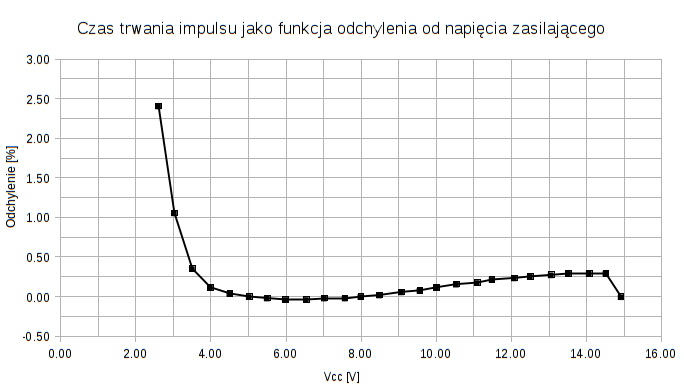
\includegraphics[width=1.1\textwidth]{charak1}
  \caption{}
\end{figure}
Na podstawie rys. 3 możemy wnioskować, iż czas trwania impulsu utrzymuje się na względnie stałym poziomie - maksymalne pojedyncze odchylenie wynosi
$2.41\%$, natomiast dla przeważającej liczby pomiarów odchylenie nie przekracza $0.5\%$.
\pagebreak
\subsection{Czas trwania impulsu a napięcie modulujące}
\begin{figure}[h]
  \centering
  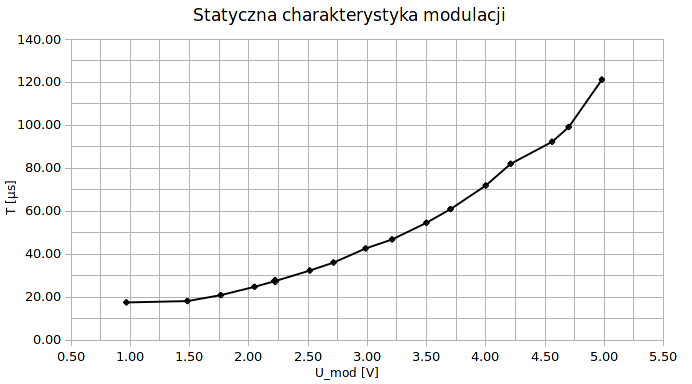
\includegraphics[width=1.1\textwidth]{charak2}
  \caption{}
\end{figure}
Na podstawie rysunku nr.4 możemy wnioskować, iż wraz ze wzrostem napięcia modulującego długość impulsów rośnie, ponieważ zmieniamy polaryzacje wejść wewnętrznych komparatorów układu (czas ładowania kondensatora wzrasta)
%%%%%%%%%%%%%%%%%%%%%%%%%%%%%%%%%%%%%%%%%%%%%%%%%%%%%%%%%%%%%%%%%%%%%%%%%%%%%%%%%%%%%%%%%%%%%%%%%%%%%%%%%%%%%%%%%%%%%%%%%%%%%%%%%%%%%%%%%%%%%%%%%%%%
\section {Wnioski}
\begin{enumerate}  
\item Czas trwania impulsu charakteryzuje się małym odchyleniem od wartości nominalnej (dla 5V-napięcia zasilania),
      zgodnie z rysunkiem nr 3 układ doskonale utrzymuje zadany czas trwania impulsu na przedziale
      napięcia zasilania od ok. 3.5V do 15V, ponieważ odchyłka od oczekiwanego czasu jest mniejsza od 0.5\%.
\item Wraz ze wzrostem napięcia modulującego długość impulsów wzrasta, na rys. 4 widać, że 
      zadaną wartość długosci impulsów (50us) otrzymujemy dla napięcia modulujcego będącego w przedziale od
      3.25V do 3.5V.
\item Układ monostabilny charakteryzuje się jednym stanem stabilnym, drugi stan trwa tylko przez określony czas, zależny od wartości elementów układu. Po upływie tego stanu samoczynnie  wraca  do  stanu  stabilnego.
\end{enumerate}
\end{document}
